%!TEX root = main.tex

\chapter{Propositional Formulas and Models}

In this chapter, we begin the discussion of propositional logic. We will define how propositional formulas look, what is a model in propositional logic and we will also discuss some special forms of formulas.

Propositional logic is the more basic type of logic (and predicate logic is an extension of propositional logic in a sense).  Propositional formulas (propositions) are created from so-called \emph{propositional variables} that represent an atomic fact which can either be true or false. These propositional variables can only be connected by common logic connectives ($\to$, $\lequiv$, $\land$, $\lor$, $\neg$). Logical formulas can additionally use parentheses to indicate the order of application of connectives. While the propositional formulas are simple compared to formulas in other types of logic, they are still useful. One of the most important problems in propositional logic and in computer science in general is the satisfiability of propositional formulas (SAT). Many other NP-complete problems are often solved by transformation to the SAT problem and using one of the existing SAT solvers.

\section{Syntax of Propositional Logic}

The set of propositional variables is often called $\Prop$ and the variables themselves are usually named $p, q, r, s$ or $p_0, p_1, \dots, q_0, q_1$, or similarly. Now we can formally define a propositional formula (over $\Prop$).

\begin{definition}
Let $\Prop$ be the set of propositional variables, then
\begin{enumerate}
  \item Every propositional variable from $\Prop$ is a propositional formula.
  \item If $\varphi$ and $\psi$ are propositional formulas, then $(\varphi \to \psi), (\varphi \land \psi), (\varphi \lor \psi), (\varphi \lequiv \psi)$, and $(\neg \varphi)$ are propositional formulas.
  \item Every propositional formula is created by finite application of the two rules above.
\end{enumerate}
\end{definition}

The last part of the definition ensures that every formula is finite; this also means that each formula can contain only a finite number of distinct variables. The set of propositional variables used in a formula $\varphi$ will be denoted as $\Var(\varphi)$. On the other hand, the set of all propositional formulas using only variables from a set $\Prop$ will be denoted as $\VF_\Prop$.

Formulas are thus strings created from propositional variables, logical connectives, and parentheses, that fulfill the conditions in the definition above. A substring of such a string that also fulfills the conditions is called a \emph{sub-formula}. 

The formal definition of formula dictates the use of parentheses around every sub-formula, which can be rather cumbersome. Therefore, we define priorities of the logical connectives and can thus omit some of the parentheses. The standard priorities are such that negation ($\neg$) has the highest priority (therefore parentheses around $(\neg \varphi)$ can always be omitted), conjunction and disjunction ($\lor, \land$) have ``middle'' priority, and implication and equivalence ($\to, \lequiv$) have the lowest priority. Therefore, we can write $\varphi \land \psi \to \neg \varphi \lor \xi$ instead of $((\varphi \land \psi) \to ((\neg \varphi) \lor \xi))$. 

Each formula can be also represented by a so-called \emph{formation tree}, which is a finite ordered tree, whose nodes are labeled with propositions. The leaves are labeled with propositional variables. If a node has label $(\neg \varphi)$, it has a single child labeled with $\varphi$, and if a node has label $(\varphi \to \psi), (\varphi \land \psi), (\varphi \lor \psi),$ or $(\varphi \lequiv \psi)$, it has two children, the left one with label $\varphi$, and the right one with label $\psi$. For example, the formula $p \land q \to \neg (p \lor s)$ is represented by the formation tree on the right.
\begin{marginfigure}[-4\baselineskip]
\centering
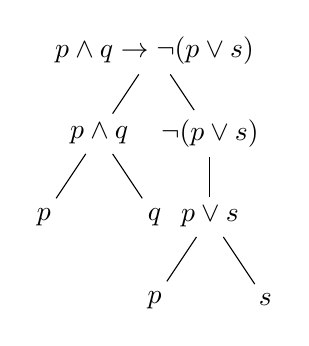
\begin{tikzpicture}[sibling distance=4em, level distance=3em]
  \node {$p \land q \to \neg (p \lor s)$}
    child { node {$p \land q$} 
      child {node {$p$}}
      child {node {$q$}} }
    child { node {$\neg (p \lor s)$}
    	child {node {$p \lor s$}
    		child {node {$p$}}
      	child {node {$s$}}}
     };
\end{tikzpicture}
\caption{The formation tree representing the formula $p \land q \to \neg (p \lor s)$.}
\end{marginfigure}

It is simple to show (by induction on the number of nested parentheses) that each formula is associated with a unique formation tree. 

\section{Semantics of Propositional Logic}

Once we have a formal definition of formulas (the syntax of propositional logic), we can define their semantics (what formulas mean). The propositional variables represent atomic statements that can have one of two truth values -- either 0 (false) or 1 (true). The truth value of a whole proposition is then given by the truth values of the variables and by the semantics of the logical connectives, which are given in Table~\ref{tab:prop_semantics} bellow.

\begin{table}[h]
\centering
\caption{The semantics of logical connectives}
\label{tab:prop_semantics}
\begin{tabular}{cc|ccccc}
\toprule
$p$ & $q$ & $\neg p$ & $p \lor q$ & $p \land q$ & $p \to q$ & $p \lequiv q$ \\
\midrule
0 & 0 & 1 & 0 & 0 & 1 & 1 \\
0 & 1 & 1 & 1 & 0 & 1 & 0 \\
1 & 0 & 0 & 1 & 0 & 0 & 0 \\
1 & 1 & 0 & 1 & 1 & 1 & 1 \\
\bottomrule
\end{tabular}
\end{table}

We can also consider the table above as a definition of Boolean functions $\lor_1, \land_1, \to_1, \lequiv_1,$ and $-_1$, which implement the logical connectives. We will use these functions in cases where it is needed (e.g. while talking about truth values of propositions). More generally, any propositional formula with $n$ variables defines a Boolean function $f: \{0,1\}^n \to \{0,1\}$ (later, we will also see that any Boolean function can be expressed using a propositional formula).

We also define two special logical formulas: the formula $\top \equiv p \lor \neg p$, which is always true, and the formula $\bot \equiv p \land \neg p$ which is always false.

We can now define truth assignments and the truth value of a formula more formally.

\begin{definition}
A \emph{truth assignment} is a function $v: \Prop \to \{0,1\}$, that is $v \in \fset{\Prop}{2}$.

A \emph{truth value} $\bar{v}(\varphi)$ of a propositional formula $\varphi$ for a truth assignment $v$ is defined inductively as:
	\begin{itemize}
		\begin{minipage}{0.5\textwidth}
		\item $\bar{v}(p) = v(p)$ if $p \in \Prop$
		\item $\bar{v}(\neg \varphi) = -_1(\bar{v}(\varphi))$ 
		\item $\bar{v}(\varphi \lor \psi) = \lor_1(\bar{v}(\varphi),\bar{v}(\psi))$ 
		\end{minipage}
		\begin{minipage}{0.5\textwidth}
		\item $\bar{v}(\varphi \land \psi) = \land_1(\bar{v}(\varphi),\bar{v}(\psi))$ 
		\item $\bar{v}(\varphi \to \psi) = \to_1(\bar{v}(\varphi),\bar{v}(\psi))$ 
		\item $\bar{v}(\varphi \lequiv \psi) = \lequiv_1(\bar{v}(\varphi),\bar{v}(\psi))$ 
		\end{minipage}
	\end{itemize}
\end{definition}

We can easily show (by induction on the structure of the formula) that the truth value of a formula $\varphi$ depends only on the truth assignment of variables from $\Var(\varphi)$.

A proposition $\varphi$ over $\Prop$ is \emph{true in (satisfied by) an assignment} $v\in \fset{\Prop}{2}$, if $\bar{v}(\varphi) = 1$. In such a case, $v$ is called a \emph{satisfying assignment} for $\varphi$; we denote this fact $v \vDash \varphi$. If the formula is true for all assignments $v \in \fset{\Prop}{2}$, we say that it is \emph{valid (a tautology)} and denote the fact as $\vDash \varphi$. On the other hand, if there is no assignment for which the formula is true, it is called \emph{unsatisfiable (a contradiction)}. A formula $\varphi$ is \emph{independent (a contingency)} if it is neither a tautology nor a contradiction, i.e. there are two assignments $v_1, v_2 \in \fset{\Prop}{2}$, such that $\bar{v}_1(\varphi) = 1$ and $\bar{v}_2(\varphi) = 0$. Finally, a formula is \emph{satisfiable} if there is a truth assignment in which it is true.

A truth assignment of $\Prop$ is also called a model of the language $\Prop$. The set of all models of $\Prop$ is denoted as $M(\Prop)$, and, obviously $M(\Prop) = \fset{\Prop}{2}$. A proposition $\varphi$ over $\Prop$ is valid in a model $v \in M(\Prop)$ if $\bar{v}(\varphi) = 1$. Then we also say that $v$ is a model of $\varphi$, denoted as $v \vDash \varphi$. $M^\Prop(\varphi) = \{v \in M(\Prop) | v \vDash \varphi\}$ is the \emph{class of all models} of $\varphi$. A formula is valid if it is true in every model of the language, it is unsatisfiable if it does not have a model, and is satisfiable if it has a model. It is independent if it is true in some model of the language and false in some other one. Formulas $\varphi$ and $\psi$ are logically equivalent ($\varphi \sim \psi)$ if $M^\Prop(\varphi) = M^\Prop(\psi)$.

The last two paragraphs say basically the same thing; the difference is that in the latter one we use the notion of a model, which is central to logic. The notion of models and sets of models will be important later, and ``model'' is one of the key terms in logic.

In the definition of propositions, we used 5 different logical connectives. However, if we take a look at the table with their semantics, we may notice that, for example, $p \to q$ is equivalent to $\neg p \lor q$. Therefore, even without using implication ($\to$) we can still express everything we could with it. More formally, for every formula $\varphi \in \VF_\Prop$, there is an equivalent formula $\varphi'$ that does not use implication. Moreover, we can notice that $p \lequiv q$ is equivalent to $(p \to q) \land (q \to p)$, therefore we even do not need equivalence, and every formula can be written using only negation, conjunction, and disjunction ($\neg, \land, \lor$). This feature of a set of connectives can be defined more formally.

\begin{definition}
A set of connectives is \emph{adequate} if they can express any Boolean function by some proposition formed from them.
\end{definition}

We have already discussed that the set $\{\neg, \land, \lor\}$ is adequate. We can also show that the set $\{\to, \neg\}$ is adequate; the easiest way to do that is to realize that $(p \land q) \sim \neg (p \to \neg q)$ and $(p \lor q) \sim (\neg p \to q)$. 

Generally we can also define custom connectives. For example, the so-called Shaffer stroke (NAND) is defined as $p \uparrow q \sim \neg (p \land q)$, and the Pierce arrow (NOR) is defined as $p \downarrow q \sim \neg (p \lor q)$. Interestingly, both $\{\uparrow\}$ and $\{\downarrow\}$ are adequate sets. This is an important fact for the construction of logical circuits as we can use a logical gate of only one kind (either NAND or NOR) to express any Boolean function.

\section{Normal Forms}

There are also special forms of formulas, which are often used. Among the most common ones are so-called conjunctive and disjunctive normal forms. In order to define these two forms, we first need to define a literal. A \emph{literal} is a propositional variable or its negation. For example, if $\Prop = \{p, q\}$ then all the literals we can construct over $\Prop$ are $\{p, \neg p, q, \neg q\}$. A formula is in conjunctive normal form (CNF) if it is a conjunction of disjunctions of literals. Disjunctions of literals are also called \emph{clauses}, therefore we can also say that a CNF formula is a conjunction of clauses. On the other hand, a formula is in disjunctive normal form (DNF) if it is a disjunction of conjunctions of literals. So, for example, $(p \lor \neg q \lor r) \land (p \lor q) \land (\neg p \lor q \lor r)$ is a formula in CNF and$(\neg p \land q \land \neg r) \lor (\neg p \land \neg q) \lor (p \land \neg q \land \neg r)$ is a formula in DNF (and, moreover a negation of the previous one in CNF). 

Now we would like to show that for every formula there is an equivalent formula in CNF and another equivalent formula in DNF. To this end, we will need the following set of rules, which can be proven by checking the truth table of the propositional connectives: 

\begin{enumerate}
  \item $(\varphi \to \psi) \sim (\neg \varphi \lor \psi), (\varphi \lequiv \psi) \sim ((\neg \varphi \lor \psi) \land (\neg \psi \lor \varphi))$
  \item $\neg \neg \varphi \sim \varphi, \neg (\varphi \land \psi) \sim (\neg \varphi \lor \neg \psi), \neg (\varphi \lor \psi) \sim (\neg \varphi \land \neg \psi)$
  \item $(\varphi \lor (\psi \land \chi)) \sim ((\psi \land \chi)  \lor \varphi) \sim ((\varphi \lor \psi) \land (\varphi \lor \chi))$
  \item $(\varphi \land (\psi \lor \chi)) \sim ((\psi \lor \chi)  \land \varphi) \sim ((\varphi \land \psi) \lor (\varphi \land \chi))$
\end{enumerate}

We can also easily show (again by induction on the structure of the formula) that if we have a formula $\varphi'$ which is obtained from $\varphi$ by replacing some occurrences of its sub-formula $\psi$ with an equivalent sub-formula $\psi'$, then $\varphi \sim \varphi'$.

And finally, we can show the following theorem. 

\begin{theorem}
For every formula $\varphi$ over $\Prop$, there are formulas $\varphi_C$ and $\varphi_D$ such that $\varphi_C$ is in CNF, $\varphi_D$ is in DNF and $\varphi \sim \varphi_C$ and $\varphi \sim \varphi_D$.
\end{theorem}
\begin{proof}
The propositions $\varphi_C$ and $\varphi_D$ can be obtained from $\varphi$ by applying the rules 1 to 4 mentioned above. 
\end{proof}

The discussion above shows one of the ways to obtain formulas in CNF and DNF equivalent to a given formula. We can in fact apply the rules in the order in which they are presented. First, we remove all the implications and equivalences by using rule no. 1. Then we move all negations to the literals (i.e. there are no negations outside of parentheses), using rule no. 2 and, finally, we repeatedly apply rules no. 3 and 4 to obtain the CNF and DNF. 

This syntactic approach is not the only one to obtain CNF/DNF from a given formula. We can also construct the truth table of the formula and then read the CNF/DNF almost directly from the table. We will show a more general approach here: we will construct CNF and DNF formulas $\varphi_C$ and $\varphi_D$ such that $M^\Prop(\varphi_C) = M^\Prop(\varphi_D) = K \subseteq M(\Prop)$, for a given finite set of truth assignments $K$ over a finite $\Prop$.

Before we show the construction, we will define the notion of $p^t$ for a variable $p$ and a truth value $t$ as $$ p^t = \twopartdef{p}{t = 1}{\neg p}{t = 0}\,.$$ 

Now we can easily see that for a single assignment $v \in K$, the set of models of the formula $\Land_{p \in \Prop} p^{v(p)}$ contains only $v$. For a set of assignments $K$, we can just make a disjunction over all assignments in $K$ (remember $K$ is a finite set). Therefore, $$M(\Lor_{v \in K}\Land_{p \in \Prop}p^{v(p)}) = K\,.$$ Thus we have constructed a formula in DNF whose models are exactly the set $K$. 

Constructing a formula $\varphi$ in CNF such that $M(\varphi) = K$ for some given finite $K$ is slightly more complex. However, we can use the fact that the negation of a formula in DNF is a formula in CNF. Negating a formula in CNF/DNF means changing all the conjunctions to disjunctions and vice versa and changing all literals to the complementary ones (i.e. changing $p$ to $\neg p$ and vice versa). So, we start by creating a formula $\neg \varphi$ in DNF for the set $\fset{\Prop}{2} \setminus K$ according to the approach above. Then we negate the formula, thus obtaining $\varphi$ in CNF such that $M(\varphi)=K$. Following these two steps we obtain the CNF formula $$\varphi = \Land_{v \in \fset{\Prop}{2} \setminus K}\Lor p^{-_1v(p)}$$ such that $M(\varphi) = K$.

If we want to use this approach to create a formula in CNF or DNF equivalent to a formula $\varphi$, we simply choose $K=M(\varphi)$. This description also shows that any Boolean function $f$ (i.e. function $f: \{0,1\}^n \to \{0,1\}$) can be expressed as a proposition. We can choose $K = \{v | f(v) = 1\}$. 

Both the techniques described above lead to an equivalent formula in CNF/DNF. The table-based method is typically used only for formulas with lower number of variables, as the size of the table for a formula with $n$ variables is $2^n$.

\section{Logical theories}

In mathematics, we often need to work in theories -- we assume that some facts are true (the axioms of the theory) and are interested in which other facts are true. Therefore, in logic, we define a \emph{propositional theory over the language $\Prop$} as a set of propositions from $\VF_\Prop$. These propositions are called \emph{axioms}. An assignment $v \in M(\Prop)$ is a \emph{model of theory $T$} ($v \vDash T$), if all axioms of $T$ are true in $v$. Similarly to formulas, we define the \emph{class of models of $T$} as $M(T) = \{v \in M(\Prop) | v \vDash \varphi \text{ for all } \varphi \in T\}$. A finite theory is equivalent to a conjunction of its axioms. We will also write $M(T, \varphi)$ as a shortcut for $M(T \cup \{\varphi\})$.

We can now re-define semantic concepts with respect to a theory. Let $T$ be a theory over $\Prop$ and $\varphi$ a proposition over $\Prop$. We say that \emph{$\varphi$ is true (valid) in $T$} ($T\vDash \varphi$) it if is true in every model of $T$. In such a case, we also say that $\varphi$ is a (semantic) consequence of $T$. A formula $\varphi$ is \emph{unsatisfiable (contradictory) in $T$ (inconsistent with $T$)}, if it is false in every model of $T$. It is \emph{independent (a contingency) in T}, if it is true is some model of $T$ and false in some other model of $T$, and \emph{satisfiable in $T$} if it is true in some model of $T$. Two propositions $\varphi$ and $\psi$ are \emph{equivalent in $T$ ($T$-equivalent)} ($\varphi \sim_T \psi$), if for every model $v \in M(T)$, $v \vDash \varphi$ if and only if $v \vDash \psi$. For an empty theory ($T = \emptyset$), or for a theory where all axioms are tautologies, the re-definitions in this paragraph are equivalent to the definitions mentioned earlier.

The concepts defined above can also be expressed using the sets of models. For example $T \vDash \varphi$ is the same as $M(T) \subseteq M(\varphi)$, and $\varphi \sim_T \psi$ is equivalent to $M(T, \varphi) = M(T, \psi)$.

For each theory, we define its consequences as the set of all propositions that are true in the theory -- $\cons^\Prop(T) = \{\varphi\ | \varphi \in \VF_\Prop, T \vDash \varphi \}$. Now, if we have two theories $T$ and $T'$, such that $T \subseteq T'$ over $\Prop$, we can prove that $T \subseteq \cons^\Prop(T) = \cons^\Prop(\cons^\Prop(T)) \subseteq \cons^\Prop(T')$. The first part says, that each axiom of $T$ is always a consequence of $T$. This makes sense, as an axiom of $T$ is by definition true in all models of $T$. The next part says, that the consequences of consequences of $T$ are still the original consequences. However, this is also simple to show. Obviously, $M^\Prop(T) = M^\Prop(\cons(T))$ and therefore also $\cons^\Prop(T) = \cons^\Prop(\cons^\Prop(T))$ by the definition of a consequence. Finally, if we have a formula $\varphi$ which is valid in all models of $T$, then $\varphi$ is also valid in all models of $T'$ ($T \subseteq T'$) as each model of $T'$ also must be a model of $T$. Therefore $\cons^\Prop(T) \subseteq \cons^\Prop(T')$.

Similarly, if we have propositions $\varphi, \varphi_1, \varphi_2, \dots \varphi_n$ over $\Prop$, we can show that $\varphi \in \cons^\Prop(\{\varphi_1, \dots, \varphi_n\})$ if and only if $\vDash (\varphi_1 \land \dots \land \varphi_n) \to \varphi$.

A theory $T$ over $\Prop$ is \emph{inconsistent (unsatisfiable)} if $T \vDash \bot$, otherwise $T$ is \emph{consistent (satisfiable)}. A theory is consistent if and only if it has a model. A theory is \emph{complete} if it is consistent and $T\vDash \varphi$ or $T \vDash \neg \varphi$ for every $\varphi \in \VF_\Prop$, i.e. there are no independent propositions in $T$. This is also equivalent to the fact that $T$ has exactly one model (if $T$ had two models $v_1$ and $v_2$, then there would be a propositional variable $p$, such that $v_1(p) \neq v_2(p)$ and therefore the formula $p$ is true in one of the models and false in the other one, thus $p$ is independent). In mathematics, we very often create new theories by adding axioms to other theories. Such new theories are called extensions of the original theories. More formally, a theory $T$ over $\Prop$ is an \emph{extension} of $T'$ over $\Prop'$, if $\Prop' \subseteq \Prop$ and $\cons^{\Prop'}(T') \subseteq \cons^\Prop(T)$. An extension is \emph{simple} if $\Prop = \Prop'$, and it is \emph{conservative} if $\cons^{\Prop'}(T') = \cons^\Prop(T) \cap \VF_{\Prop'}$. Two theories $T$ and $T'$ are equivalent, if $T$ is an extension of $T'$ and vice versa.

Although we motivated the notion of extension by adding new axioms, it is defined more generally using the sets of consequences of the theory. This abstracts from the particular axioms and considers all equivalent theories the same. The notion of extension can also be expressed with the sets of models, if both theories $T$ and $T'$ are over the same language $\Prop$. In such a case $T$ is an extension of $T'$ if and only if $M^\Prop(T) \subseteq M^\Prop(T')$, and the two theories are equivalent if $M^\Prop(T)=M^\Prop(T')$.

We will conclude this section with the discussion about the number of nonequivalent propositions and theories over a finite language $\Prop$. We defined two formulas or theories to be equivalent if they have the same sets of models. Therefore, if we want to compute the number of non-equivalent theories/formulas, we can instead compute the number of sets of models. So, if $|\Prop| = n$, then there are $2^{2^n}$ non-equivalent formulas (theories) over $\Prop$, as there are $2^n$ different assignments, and every set of assignments represents a formula (remember, we know how to write that formula in CNF/DNF) or a theory. 

Using similar reasoning, we can show how many nonequivalent valid (or contradictory -- the number is the same) propositions are there in a theory. A valid proposition is true in all models of $T$, therefore there are $2^n-|M(T)|$ assignments where a valid proposition can be (but does not have to be) true. This means there are $2^{2^n-|M(T)|}$ valid (and contradictory) propositions in $T$. Every proposition is either valid, contradictory or independent, therefore there are $2^{2^n} - 2\times2^{2^n-|M(T)|}$ nonequivalent independent propositions in $T$. A theory has $2^{|M(T)|}$ simple extensions. One of these is contradictory (the set of models of an extension is a subset of the models of the original theory), and the same theory has $|M(T)|$ simple complete extensions (those correspond to single-element subsets of $M(T)$).

Instead of talking about nonequivalent propositions, we can also discuss T-nonequivalent propositions. There are $2^{|M(T)|}$ T-nonequivalent propositions (we now consider only subsets of $M(T)$ as the possible sets of models for the proposition). One of them is valid and one is contradictory in $T$, thus the number of $T$-nonequivalent propositions independent in $T$ is $2^{|M(T)|}-2$.

The fact that we can use the number of subsets of models while computing the number of nonequivalent theories or formulas is more formally explained by so-called Lindenbaum-Tarski algebra. For a consistent theory $T$ over $\Prop$, we can define operations $\neg, \land, \lor, \bot, \top$ on the quotient set $\VF_\Prop/\sim_T$ by using representatives, e.g. $[\varphi]_{\sim_T} \land [\psi]_{\sim_T} = [\varphi \land \psi]_{\sim_T}$. Then $AV^\Prop(T) = \langle \VF_\Prop/\sim_T, \neg, \land, \lor, \bot, \top \rangle$ is the \emph{Lindenbaum-Tarski algebra for $T$}. Since $\varphi \sim_T \psi$ if and only if $M(T, \varphi) = M(T, \psi)$ then $h([h]_{\sim_T}) = M(T, \varphi)$ is an injective function $h: \VF_\Prop \to \powerset(M(T))$. If $M(T)$ is finite then $h$ is additionally surjective, and therefore $AV$ is isomorphic to the algebra of sets $\powerset(M(T))$.


\section{Satisfiability of Propositional Formulas}

The problem of satisfiability of logical formulas is one of the central problems in computer science. The general question posed by the problem is whether a given formula in CNF is satisfiable. In general, this problem is NP-complete\sidenote{A problem $c$ is NP-complete, if it is NP and if any other NP problem is reducible to $c$ in polynomial time. A problem is NP if given a candidate solution, we can check in polynomial time that it is indeed a solution. A problem $p$ is reducible to $c$ in polynomial time, if we can transform each instance of $c$ into an instance of $p$ in polynomial time.}, which means that we do not know any polynomial-time algorithm to solve it. However, there are some special types of formulas for which SAT can be solved in polynomial time. In this section, we will discuss such formulas and show the algorithms that solve SAT for these. We will also briefly discuss local search algorithms for SAT, and describe the complete (but generally exponential) DPLL~\sidenote{The name of the procedure is derived from the names of its authors -- it was introduced in 1962 by Martin Davis, George Logemann and Donald W. Loveland as an extension of an earlier procedure by Martin Davis and Hilary Putnam.} procedure.

The first class of formulas are so called 2-CNF. A formula is in \emph{$k$-CNF} if it is a conjunction of clauses and each of the clauses contains at most $k$ literals. The SAT problem for $k$-CNF formulas is called $k$-SAT. The $k$-SAT problem is NP-complete for $k>2$, however for $k=2$ it can be solved in polynomial time using the so-called implication graph of the formula. 

\begin{definition}
Let $\varphi$ is a formula over $\Prop$ in 2-CNF, $\varphi \equiv \Land_{i=1}^j (l_{i1} \lor l_{i2}) \land \Land_{i=j+1}^k l_{i}$. The \emph{implication graph} of $\varphi$ is an oriented graph $G_\varphi = (V, E)$, where the set of vertices is $$V = \{p | p \in \Prop\} \cup \{\neg p | p \in \Prop\}$$ and the set of edges is $$E = \{(\bar{l}_{i1}, l_{i2}) | 1 \leq i \leq j\} \cup \{(\bar{l}_{i2}, l_{i1}) | 1 \leq i \leq j \} \cup \{(\bar{l}_i, l_i) | j + 1 \leq i \leq k\}\,.$$
\end{definition}

In the implication graph, the set of vertices corresponds to all literals from variables in $\Var(\varphi)$ and each clause in the formula is represented as one or two edges. For a clause $l_1 \lor l_2$, we include two edges (implications) $\bar{l}_1 \to l_2$ and $\bar{l}_2 \to l_1$. These two implications are logically equivalent to the clause. For a \emph{unit clause} $l$ (a clause with only a single literal), we include a single edge $\bar{l} \to l$; this is also equivalent to $l$. The implication graph thus contains the 2-CNF formula written as implications between its literals. The implication graph of a formula can be constructed in a time linear in the length of the formula.

Let us now assume that a truth assignment $v \in \fset{\Prop}{2}$ satisfies a formula $\varphi$. In such a case, in every strongly connected component\sidenote{In a strongly connected component, there is an oriented path between every pair of vertices.} in $G_\varphi$, all the literals have the same truth value. Otherwise there would be an implication which is not true in the assignment, which contradicts the fact that the whole formula is true in the assignment\sidenote{Assume that literals $l_1$ and $l_n$ are in the same strongly connected component and that $v(l_1) = 1$ and $v(l_n) = 0$. There is a chain of implications $l_1 \to l_2, l_2 \to l_3, \dots, l_{n-1} \to l_n$, at least one of these must be $1 \to 0$ and therefore false.}. This also means that if we have a satisfying assignment for $\varphi$, none of the strongly connected components contain both a literal and its negation. 

Can we use the implication graph of a formula to obtain a satisfying truth assignment? Indeed we can, but only if none of the strongly connected components contain a pair of complementary literals. In such a case, we can contract each of the strongly connected components into a single vertex (thus obtaining a graph $G_\varphi^*$). Such a graph would be acyclic and therefore has a topological ordering $<$. We create an assignment $v$ in a few steps: for every unassigned component in increasing order of $<$, we assign 0 to all its literals and 1 to all the complementary literals in the graph (they would in fact also form an strongly connected component). Such an assignment is satisfying for $\varphi$. If not, $G_\varphi^*$ would contain edges $p \to q$ and $\bar{q}\to\bar{p}$ with $v(p) = 1$ and $v(q) = 0$, but that contradicts the order of assignments as $p < q$ and $\bar{q} < \bar{p}$.

The discussion above can be summarized in the theorem bellow.

\begin{theorem}
Proposition $\varphi$ in 2-CNF is satisfiable if and only if no strongly connected component of its implication graph $G_\varphi$ contains a pair of complementary literals.
\end{theorem}

As the implication graph can be constructed in linear time and the strongly connected components can also be found in linear time, the 2-SAT problem can be solved in linear time.

Another class of formulas where SAT can be solved in polynomial time are conjunctions of clauses with at most one positive literal. Such clauses are called Horn clauses, and such formulas are called Horn formulas. The problem of satisfiability of Horn formulas is called Horn-SAT.

The Horn clauses can also be interpreted as implications. The Horn clause $(\neg p_1 \lor \neg p_2 \lor \dots \lor \neg p_n \lor q)$ is equivalent to the implication $(p_1 \land p_2 \land \dots \land p_n) \to q$.

Deciding whether a Horn formula $\varphi$ is satisfiable or not is simple, and can be done using the following algorithm:

\begin{enumerate}
  \item If $\varphi$ contains a pair of unit clauses $l$ and $\bar{l}$ (a pair of complementary literals) it is not satisfiable.
  \item If $\varphi$ contains a unit clause $l$, assign 1 to $l$, remove all clauses containing $l$, remove $\bar{l}$ from all clauses, and continue from the start.
  \item If $\varphi$ does not contain a unit clause, it is satisfied by assigning 0 to all remaining propositional variables.
\end{enumerate}

The first step of the algorithm is obviously correct, as $p \land \neg p$ is a contradiction, and the last step follows from the form of Horn formulas, as each of the remaining clauses contains at least one negative literal. It remains to show that the second step (also called \emph{unit propagation}) is also correct. The formula $\varphi$ can be satisfied only if each of its clauses is true, and therefore the unit clause $l$ must also be true. Once we assign 1 to $l$, we can remove all the clauses that contain $l$ (these are already satisfied) and we can also remove $\bar{l}$ from all the remaining clauses as $\bar{l}$ is 0, and therefore the clauses need to be satisfied by other literals.

This shows that Horn-SAT can be solved in polynomial time. The direct implementation of the algorithm described above is quadratic, however there are even linear implementations.

We already mentioned that there are no polynomial algorithms for the SAT problem in general, but we can use some local search algorithms to attempt to solve the problem. For example, the GSAT algorithm starts with a random truth assignment. If this assignment satisfies the formula, the algorithm ends. Otherwise it flips the truth value for one of the variables -- it chooses the variable whose change leads to the smallest number of unsatisfied clauses in the new assignment. There is a small chance to change a random variable (this allows the algorithm to escape local minima in the number of unsatisfied clauses). The WalkSAT algorithm works in a similar way, but instead of picking a variable from the whole formula, it first selects a random unsatisfied clause and picks a variable from it which minimizes the number of previously satisfied clauses that become unsatisfied by the change. It also has a small chance to pick a variable at random. 

While none of these algorithms can guarantee that they will find a satisfying assignment if one exists, they are very fast, and very often can indeed find a satisfying assignment.

A complete algorithm (which will always find an assignment, if one exists) can be implemented using backtracking and testing all possible assignments, however, such an algorithm is generally exponential. 

The DPLL procedure implements this kind of backtracking with some improvements. It first removes all clauses that are tautologies, then if a clause becomes empty during the run of the algorithm, it indicates that the current partial assignment cannot satisfy the formula and the DPLL procedure fails. After these simple steps, the DPPL procedure simplifies the formula using unit propagation and so-called \emph{pure literal elimination}\sidenote{if a literal $l$ is only positive or only negative in the formula, it can be assigned such value $v(l) = 1$ and all the clauses containing it can be removed}. If none of the previous steps can be applied, the DPLL procedure uses a splitting rule: it selects a literal and tries to call the DPLL procedure twice, once for each possible truth assignment of that literal. If at least one of these calls succeeds, the formula is satisfiable.

\chapter{Formal Proof Systems}

Up to now, we have mostly discussed the semantics of propositional logic, and have also defined many different terms semantically using the notions of truth assignments and models. We have defined a consequence of a theory as a formula that is true in all models of the theory. However, in mathematics, we usually do not check all possible models of a theory in order to tell whether a given formula is a consequence or not. Instead, we prove the formula from the axioms of the theory. 

In this chapter, we will formalize the notion of proof as a syntactical method that can be used to prove formulas in propositional logic. The formalization will be called a proof system, and, informally, a proof system is a collection of syntactical rules that provide a proof of a given formula in a given theory. The proof is then a finite object that can be built from the axioms of the theory, and if a formula has a proof, it can be found algorithmically. 

There are many different proof systems, among them are the tableau method, Hilbert systems and Gentzen systems. We will discuss the tableau method in detail later and we will also briefly mention Hilbert systems. However, a proof system can only be useful, if any formula proved by the system is also valid, and vice versa, if every valid formula can be proven. These two features of a proof system are called soundness and completeness. 

\section{Tableau Method}

The tableau method is a proof system, where the proof (tableau) of a formula $\varphi$ in a theory $T$ is a binary labeled tree representing a search for a model of $T$ where $\varphi$ is not true (a counterexample). If the search fails, the formula is proved and in such a case the tableau is finite. In case there is a counterexample of $\varphi$, the tableau can be infinite and there is a branch in the tree that provides the counterexample.

In tableau methods, we assume a fixed and countable language $\Prop$; in this case, also every theory over $\Prop$ is countable.

We already mentioned that every tableau is a labeled binary tree. The nodes in the tree are labeled by \emph{entries}, which are formulas with a \emph{sign} $T$/$F$ that represent the assumption that the formula is true ($T$) or false ($F$). The tree will be constructed using \emph{atomic tableaux} and a set of rules. For a propositional variable $p$ and propositions $\varphi, \psi$, the atomic tableaux are given in the figure bellow.

\begin{figure*}[ht]
\centering
\begin{minipage}{\textwidth}
\begin{tabular}{|c|c|c|c|c|c|}
\hline
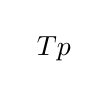
\begin{tikzpicture}[sibling distance=3em, level distance=3em]
  \node {$Tp$};
\end{tikzpicture} &
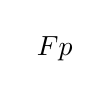
\begin{tikzpicture}[sibling distance=3em, level distance=3em]
  \node {$Fp$};
\end{tikzpicture} &
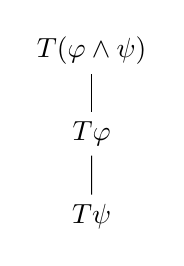
\begin{tikzpicture}[sibling distance=3em, level distance=3em]
  \node {$T (\varphi \land \psi)$}
    child { node {$T \varphi$} 
      child {node {$T \psi$}}};
\end{tikzpicture} &
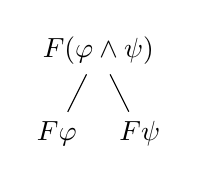
\begin{tikzpicture}[sibling distance=3em, level distance=3em]
  \node {$F (\varphi \land \psi)$}
    child { node {$F \varphi$} }
    child { node {$F \psi$}};
\end{tikzpicture} &
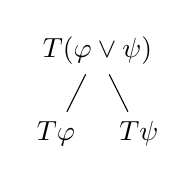
\begin{tikzpicture}[sibling distance=3em, level distance=3em]
  \node {$T (\varphi \lor \psi)$}
    child { node {$T \varphi$} }
    child { node {$T \psi$}};
\end{tikzpicture} &
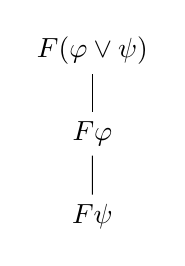
\begin{tikzpicture}[sibling distance=3em, level distance=3em]
  \node {$F (\varphi \lor \psi)$}
    child { node {$F \varphi$} 
      child {node {$F \psi$}}};
\end{tikzpicture} \\
\hline
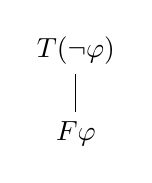
\begin{tikzpicture}[sibling distance=3em, level distance=3em]
  \node {$T (\neg \varphi)$}
    child { node {$F \varphi$} };
\end{tikzpicture} &
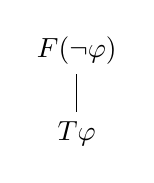
\begin{tikzpicture}[sibling distance=3em, level distance=3em]
  \node {$F (\neg \varphi)$}
    child { node {$T \varphi$} };
\end{tikzpicture} &
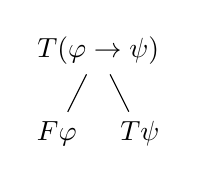
\begin{tikzpicture}[sibling distance=3em, level distance=3em]
  \node {$T (\varphi \to \psi)$}
    child { node {$F \varphi$} }
    child { node {$T \psi$}};
\end{tikzpicture} &
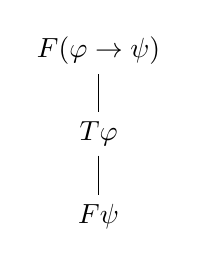
\begin{tikzpicture}[sibling distance=4em, level distance=3em]
  \node {$F (\varphi \to \psi)$}
    child { node {$T \varphi$} 
      child {node {$F \psi$}}};
\end{tikzpicture} &
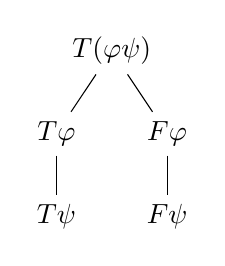
\begin{tikzpicture}[sibling distance=4em, level distance=3em]
  \node {$T (\varphi \lequiv \psi)$}
    child { node {$T \varphi$} 
    	child {node {$T \psi$}}}
    child { node {$F \varphi$} 
    	child {node {$F \psi$}}};
\end{tikzpicture} &
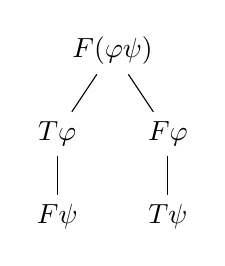
\begin{tikzpicture}[sibling distance=4em, level distance=3em]
  \node {$F (\varphi \lequiv \psi)$}
    child { node {$T \varphi$} 
    	child {node {$F \psi$}}}
    child { node {$F \varphi$} 
    	child {node {$T \psi$}}};
\end{tikzpicture} \\
\hline
\end{tabular}
\end{minipage}
\caption{The atomic tableaux}
\label{fig:prop_tableaux}
\end{figure*}

\informal{The labels in each of the tableaux show whether a formula $\varphi$ should be true ($T \varphi$) or false ($F \varphi$). The tableaux themselves then ``re-write'' the requirement in their root into more simple requirements. For example, the atomic tableau for $T(\varphi \to \psi)$ expresses that a formula $(\varphi \to \psi)$ is true (T), if $\varphi$ is false ($F \varphi$) or $\psi$ is true $T \psi$. The ``or'' is expressed by the two children. On the other hand, the atomic tableau for $F(\varphi \to \psi)$ says that $\varphi \to \psi$ is false, if $\varphi$ is true and $\psi$ is false. The ``and'' is presented by the fact, that both these facts are on a single branch.

While the atomic tableaux are based on the semantics of propositional logic, the tableau method itself is purely syntactic -- it only says how to manipulate tableaux in order to obtain the proof of a formula.}

Using the atomic tableaux, we can define tableaux in general.

\begin{definition}
A \emph{finite tableau} is a binary tree labeled with entries defined inductively as follows:
\begin{enumerate}
	\item Every atomic tableau is a finite tableau.
  \item If $P$ is an entry on a branch $V$ in a finite tableau $\tau$ and $\tau'$ is obtained by adjoining the atomic tableau for $P$ at the end of branch $V$, then $\tau'$ is also a finite tableau.
  \item Every finite tableau is formed by finite number of steps above.
\end{enumerate}

A \emph{tableau} $\tau$ is a (potentially infinite) sequence $\tau_0, \tau_1, \dots, \tau_n, \dots$  of finite tableaux such that $\tau_{n+1}$ is formed from $\tau_n$ by an application of step 2 above. Formally, $\tau = \bigcup \tau_n$.
\end{definition}

An example of a tableau is shown below. In propositional logic, we do not need to repeat the entries that we expand, therefore, we will generally use only the version on the right, where these repeated entries are removed.\sidenote{In predicate logic, some of the repeated entries need to be included in the tableau again.}

\begin{figure}[ht]
\begin{minipage}{0.5\textwidth}
\centering
\begin{tikzpicture}[sibling distance=4em, level distance=3em]
  \node(n) {$F(((p \to q) \to p) \to p)$}
    child { node {$T ((p \to q) \to p)$} 
    	child { node {$F p$} 
    		child {node {$T ((p \to q) \to p)$}
    			child {node {$F(p \to q)$}
    				child {node {$F(p \to q)$}
	    				child {node {$Tp$}
	    					child {node {$Fq$}
	    						child {node {$\otimes$}}
	    					}
	    				}
	    			}
    			}
    			child {node {$Tp$}
    				child {node {$\otimes$}}
    			}
    		}
    	}
    };
  \node[fit=(n)(n-1-1), draw] {};
  \node[fit=(n-1-1-1)(n-1-1-1-1), draw] {};
  \node[fit=(n-1-1-1-1-1)(n-1-1-1-1-1-1-1), draw] {};
\end{tikzpicture}
\end{minipage}
\begin{minipage}{0.5\textwidth}
\centering
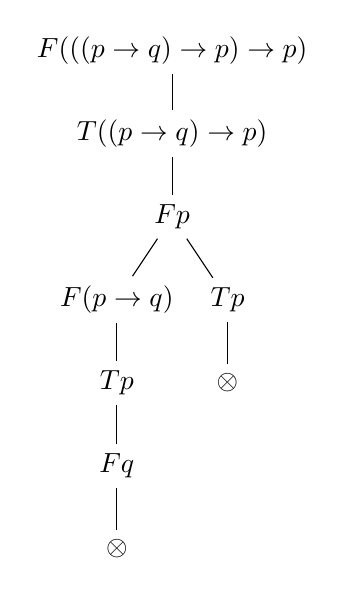
\begin{tikzpicture}[sibling distance=4em, level distance=3em]
  \node(n) {$F(((p \to q) \to p) \to p)$}
    child { node {$T ((p \to q) \to p)$} 
    	child { node {$F p$} 
  			child {node {$F(p \to q)$}
  				child {node {$Tp$}
  					child {node {$Fq$}
  						child {node {$\otimes$}}
  					}
  				}
  			}
  			child {node {$Tp$}
  				child {node {$\otimes$}}
  			}
    	}
    };
\end{tikzpicture}
\end{minipage}
\caption{Example tableau. The rectangles on the left show the atomic tableaux used. The version on the right removes the repeated entries. The symbol $\otimes$ denotes a contradictory branch.}
\label{fig:tableau_notation_proof}
\end{figure}

The definition above does not specify how to choose an entry $P$ on branch $V$ for expansion. Later, we will define systematic tableaux, where this is specified.

Before we can define the formal notion of proof using the tableau method, we first need to discuss some of the terms related to tableaux. For an entry $P$ on a branch $V$ in a tableau $\tau$, we say that \emph{$P$ is reduced on $V$} if it occurs on $V$ as a root of an atomic tableau. A \emph{branch $V$ is contradictory} if it contains entries $T \varphi$ and $F \varphi$ for some proposition $\varphi$, otherwise it is noncontradictory. A \emph{branch $V$ is finished} if it is contradictory, or every entry on $V$ is reduced on $V$. Finally, a \emph{tableau $\tau$ is finished} if every branch in $\tau$ is finished, and $\tau$ is contradictory if every branch in $\tau$ is contradictory.

A \emph{tableau proof of $\varphi$} is a contradictory tableau with the root entry $F \varphi$. A formula \emph{$\varphi$ is tableau provable} ($\vdash \varphi$) if it has a tableau proof. On the other hand, a \emph{refutation of $\varphi$ by tableau} is a contradictory tableau with the root entry $T \varphi$, and \emph{$\varphi$ is tableau refutable} it it has a tableau refutation; in this case we write $\vdash \neg \varphi$.

\informal{Why does a tableau proof of $\varphi$ start with $F \varphi$? Tableaux in fact represent systematic searches for assignments that fulfill the condition expressed by the entry in the root. Therefore, if we cannot find a truth assignment in which $\varphi$ is false (the tableau for $F \varphi$ is contradictory), then $\varphi$ must be true in all assignments, and therefore valid. The formal proof of the soundness and completeness of the tableau methods will be discussed shortly.}

\begin{figure}
\centering
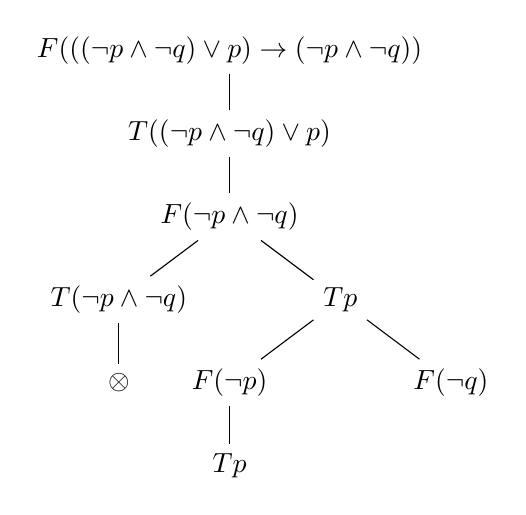
\begin{tikzpicture}[sibling distance=8em, level distance=3em]
  \node {$F(((\neg p \land \neg q) \lor p) \to (\neg p \land \neg q))$}
    child { node {$T ((\neg p \land \neg q) \lor p)$} 
    	child { node {$F (\neg p \land \neg q)$} 
    		child {node {$T (\neg p \land \neg q)$}
    			child {node {$\otimes$}}}
    		child {node {$T p$}
    			child {node {$F(\neg p)$}
    				child {node {$T p$}}}
    			child {node {$F(\neg q)$}}
    			}}
    	};
\end{tikzpicture}
\caption{Example tableau. Both left and middle branches are finished. The left one is also contradictory, while the middle one is noncontradictory. The right branch is not finished.}
\label{fig:tableau_example}
\end{figure}

Figure~\ref{fig:tableau_example} shows a tableau with the root entry $F(((\neg p \land \neg q) \lor p) \to (\neg p \land \neg q))$. The tableau has three branches. The leftmost one is contradictory, as it contains both $F (\neg p \land \neg q)$ and $T (\neg p \land \neg q)$, the middle one is finished and noncontradictory, as every entry on that branch is expanded on it, and the rightmost one is unfinished, as the entry $F (\neg q)$ is not expanded on that branch.

On the other hand, the tableau in Figure~\ref{fig:tableau_notation_proof} is a tableau proof of the proposition $(((p \to q) \to p) \to p)$, as it starts with the entry $F(((p \to q) \to p) \to p)$ and all its branches are contradictory.

We often need to work with theories, and also prove propositions in a theory. Therefore, the notion of tableau needs to be generalized to the notion of a tableau from a theory. Theories provide axioms, these are assumed to be true, and therefore the tableau from a theory $T$ can additionally contain entries of the from $T \varphi$ for an axiom $\varphi \in T$. More formally, a \emph{finite tableau from a theory $T$} is a generalized tableau with an additional rule -- if $V$ is a branch of a finite tableau (from $T$) and $\varphi \in T$, then by adjoining $T \varphi$ at the end of $V$ we obtain a finite tableau from $T$. The rest of the definitions related to tableaux can be generalized in the same way. \emph{A tableau from $T$} is a sequence $\tau_0, \tau_1, \dots, \tau_n, \dots$ of finite tableaux from $T$ such that $\tau_{n+1}$ is formed from $\tau_n$ applying rule 2 (from the definition of tableaux), or the additional rule above; formally, $\tau = \bigcup \tau_n$. A \emph{tableau proof of $\varphi$ from $T$} is a contradictory tableau from $T$ with $F \varphi$ in the root. $T \vdash \varphi$ denotes that $\varphi$ is tableau provable from $T$. A \emph{refutation of $\varphi$ by a tableau from $T$} is a contradictory tableau from $T$ with $T \varphi$ in the root. A branch $V$ of a tableau from $T$ is finished if it is contradictory, or every entry on $V$ is already reduced on $V$ and, additionally, $V$ contains $T \varphi$ for each $\varphi \in T$.

While the current definition of tableaux is enough for proving propositions in theories, here we provide a stricter definition of so-called systematic tableau. We will see later that a systematic tableau is always finished and, in case the tableau is a proof of a proposition, it is also finite. The definition prescribes the precise order of steps to use while constructing tableaux from theories -- it specifies which entry in the tableau should be expanded next and also which axiom from the theory should be added next.

\begin{definition}
Let $R$ be an entry and $T = \{\varphi_0, \varphi_1, \dots\}$ a theory. Then the \emph{systematic tableau} $\tau$ from $T$ for the entry $R$ is the result of the following construction, i.e. $\tau = \bigcup \tau_n$
\begin{enumerate}
	\item $t_0$ is the atomic tableau for $R$. Then proceed with the following steps until possible:
	\item Let $P$ be the leftmost entry in the smallest possible level of the tableau $\tau_n$ such that $P$ is not reduced on some noncontradictory branch through $P$.
	\item Let $\tau'_n$ be the tableau obtained from $\tau_n$ by adjoining the atomic tableau for $P$ to every noncontradictory branch through $P$ ($\tau'_n = \tau_n$ if no such $P$ exists).
	\item Let $\tau_{n+1}$ be the tableau obtained from $\tau'_n$ by adjoining $T \varphi_n$ to every noncontradictory branch that does not contain $T \varphi_n$ (if $\varphi_n$ does not exist, $\tau_{n+1}=\tau'_n$).
\end{enumerate}
\end{definition}

The first thing to notice is that every systematic tableau is finished. Assume we have a tableau $\tau = \bigcup \tau_n$. If there is a noncontradictory branch in $\tau$, the prefix of this branch is noncontradictory in each $\tau_n$. Therefore, the branch must contain $T \varphi_n$ for each $\varphi_n$ in $T$. Let us now assume that there is an entry $R$, such that $R$ is not reduced on a branch. However, there are only finitely many levels above $R$ in $\tau$ and therefore only finitely many entries above $R$, thus $R$ will be eventually selected in step 2 and reduced in step 3, which is a contradiction with $R$ not being reduced. So, every noncontradictory branch in the tableau is finished (it contains $T \varphi_n$ for each $\varphi_n \in T$, and every entry on the branch is reduced).

Interestingly, if tableau is used as a proof, it is not only finished, it is also finite. More specifically -- for every contradictory tableau $\tau = \bigcup t_n$, there is some $n$ such that $\tau_n$ is a contradictory finite tableau. Why? Let $S$ be the set of nodes in $\tau$ that have no pair of contradictory entries $T \varphi$, $F \varphi$ amongst their predecessors. We can imagine this set as a ``top part'' of the tableau -- the root is definitely in this set. If there is a node in the set, all of its predecessors are also there. Such a set $S$ must be finite, because otherwise, by König's lemma, the subtree of $\tau$ induced by the set $S$ would have an infinite branch (it is a finitely branching infinite tree), and therefore the tableau $\tau$ would not be contradictory. Now, since $S$ is finite, all of the nodes in $S$ belong to levels up to $m$ for some $m$. Thus every node in level $m+1$ has a pair of contradictory entries among its predecessors. We can now choose $n$ such that the top $m+1$ levels of $\tau$ are a subtree of $\tau_n$. Every branch in $\tau_n$ now contains a pair of contradictory entries and is thus contradictory.

In the construction of systematic tableaux, we extend only noncontradictory branches, therefore if a systematic tableau (from a theory) is a proof, it is finite (remember that a proof is a contradictory tableau with $F \varphi$ in its root). This is an important result; it shows that if a formula has a proof, we have an algorithm (the construction of systematic tableau) that can find the proof in a finite amount of time. It also shows that any proof from a theory depends only on a finite number of axioms from the theory. 

\section{Soundness and Completeness}

Now we want to show the soundness and completeness of the tableau method. We start with soundness and show that if a formula has a tableau proof from a theory, the formula is also valid in the theory. However, before we get to the proof, we need a definition and a lemma. We say that an \emph{entry $P$ agrees with an assignment $v$}, if $P$ is $T \varphi$ and $\bar{v}(\varphi) = 1$, or if $P$ is $F \varphi$ and $\bar{v}(\varphi) = 0$. A \emph{branch $V$ agrees with $v$} if every entry on $V$ agrees with $v$. 

\begin{lemma}
Let $v$ be a model of a theory $T$ that agrees with the root entry of a tableau $\tau = \bigcup \tau_n$. Then $\tau$ contains a branch that agrees with $v$.
\end{lemma}
\begin{proof}
We will find a sequence $V_0, V_1, \dots$ for every $n$, such that $V_n$ is a branch in $\tau_n$, $V_n \subseteq V_{n+1}$ and $V_n$ agrees with $n$. We start by verifying the lemma for all atomic tableaux, thus verifying the base of the induction. For example, if we have $v(p) = 1, v(q) = 0$ and an atomic tableau with root entry $T(p \lor q)$, then $v$ agrees with the root entry, and the branch of the tableau containing $Tp$ also agrees with $v$. We can check the other atomic tableaux similarly. Now, if $\tau_{n+1}$ is obtained from $\tau_n$ without extending $V_n$, we take $V_{n+1} = V_n$. If $\tau_{n+1}$ is obtained from $\tau_n$ by adjoining $T \varphi$ to $V_n$ for some $\varphi \in T$, let $V_{n+1}$ be this branch; then $v$ agrees with $V_{n+1}$ as $v$ is a model of $T$ (and therefore all axioms of $T$ are true in $v$). Finally, if $\tau_{n+1}$ is obtained from $\tau_n$ by adjoining the atomic tableau for some entry $P$ on $V_n$ to the end of $V_n$, we can extend $V_n$ to $V_{n+1}$ as required as $P$ agrees with $v$ and all atomic tableaux are verified. (For example, if $P = T(p\lor q)$, and $v$ is as in the example on atomic tableaux above, we obtain $V_{n+1}$ by adding $T(p \lor q)$ and $Tp$ to the end of $V_n$).
\end{proof}

Using the lemma, we can now easily prove the soundness of the tableau method in propositional logic.

\begin{theorem}[Soundness of tableau method in propositional logic]
For every theory $T$ and proposition $\varphi$, if $\varphi$ is tableau provable from $T$, then $\varphi$ is valid in $T$, i.e. $T \vdash \varphi \Rightarrow T \vDash \varphi$.
\end{theorem}
\begin{proof}
If the proposition $\varphi$ is tableau provable from $T$, there is a contradictory tableau $\tau$ from $T$ with root entry $F \varphi$. Suppose $\varphi$ is not valid in $T$. In such a case, there is a model $v$ of the theory $T$ in which $\varphi$ is false. Therefore, the root entry of the proof ($F \varphi$) agrees with $v$ and by the previous lemma, there is a branch in $\tau$ that agrees with $v$. However, that leads to a contradiction as $\tau$ is the proof of $\varphi$ from $T$, and therefore every branch of $\tau$ is contradictory and cannot agree with $v$.
\end{proof}

The soundness theorem says that whenever we have a tableau proof of a formula in a theory, the formula is valid. However, can we also prove any valid formula using the tableau method? We indeed can, as the completeness theorem states. Again, before we get to the proof of the completeness theorem, we prove a helper lemma, that formally shows that a noncontradictory branch in a finished tableau provides a counterexample.

\begin{lemma}
Let $V$ be a noncontradictory branch of a finished tableau $\tau$. Then $V$ agrees with the following assignment $v$: $$v(p) = \twopartdefotherwise{1}{Tp \text{ occurs on } V}{0}$$
\end{lemma}
\begin{proof}
We prove the lemma by induction on the structure of formulas in entries on $V$.
\begin{itemize}
 \item For an entry $T p$ on $V$, where $p$ is a propositional variable, we have $\bar{v}(p)= 1$ by definition.
 \item For an entry $F p$ on $V$, the entry $T p$ is not on $V$ as $V$ is noncontradictory, and thus we have $\bar{v}(p) = 0$ by definition.
 \item For an entry $T (\varphi \land \psi)$, we have both $T \varphi$ and $T \psi$ on $V$ as $\tau$ is finished, and by induction, we know that $\bar{v}(\varphi)=\bar{v}(\psi)=1$, therefore $\bar{v}(\varphi \land \psi)=1$ and $v$ agrees with $T (\varphi \land \psi)$.
 \item For an entry $F (\varphi \land \psi)$, we have $F \varphi$ or $F \psi$ on $V$ as $\tau$ is finished, therefore we have $\bar{v}(\varphi) = 0$, or $\bar{v}(\psi) = 0$, which leads to $\bar{v}(\varphi \land \psi) = 0$ and thus $v$ agrees with $F (\varphi \land \psi)$.
\end{itemize}

The lemma can be proven for the other possible types of entries (with $\lor, \to, \lequiv, \neg$) similarly to the last two steps for entries with $\land$.
\end{proof}

Using this lemma, it is simple to prove the completeness theorem.

\begin{theorem}
For every theory $T$ and proposition $\varphi$, if $\varphi$ is valid in $T$, then $\varphi$ is tableau provable from $T$, i.e. $T \vDash \varphi \Rightarrow T \vdash \varphi$.
\end{theorem}
\begin{proof}
We will show that an arbitrary finished tableau $\tau$ from theory $T$ with root entry $F \varphi$ is contradictory if $\varphi$ is valid in $T$.

Assume (for contradiction) that there is a noncontradictory branch $V$ in $\tau$. The previous lemma provides an assignment $v$ such that $V$ agrees with $v$, therefore also the root entry $F \varphi$ agrees with $v$ and thus $\bar{v}(\varphi) = 0$. Since $V$ is finished, it contains $T \psi$ for every $\psi \in T$, but that means that $v$ is a model of $T$ ($V$ agrees with $v$, therefore $\bar{v}(\psi) = 1$ for all $\psi \in T$). However, this contradicts the assumption that $\varphi$ is valid in $T$, therefore every branch in $\tau$ is contradictory and $\tau$ is a proof of $\varphi$ from $T$. 
\end{proof}

We can now introduce a syntactic definition of the semantic terms defined earlier and discuss the relation between the syntactic and semantic notions. First of all, we define the \emph{set of propositions provable from $T$} $$\Thm^\Prop(T) = \{\varphi | \varphi \in \VF_\Prop, T \vdash \varphi\}\,.$$ We say that a theory \emph{$T$ is inconsistent}, if $T \vdash \bot$, otherwise \emph{$T$ is consistent}. A theory \emph{$T$ is complete} if it is consistent and every proposition is provable or refutable from $T$, i.e. if $T \vdash \neg \varphi$ or $T \vdash \varphi$ for every $\varphi \in \VF_\Prop$. A theory $T$ over $\Prop$ is \emph{an extension} of $T'$ over $\Prop'$, if $\Prop' \subseteq \Prop$ and $\Thm^{\Prop'}(T') \subseteq \Thm^{\Prop}(T)$. The extension is \emph{simple} if $\Prop = \Prop'$, and it is \emph{conservative} if $\Thm^{\Prop'}(T') = \Thm^{\Prop}(T) \cap \VF_{\Prop'}$. Two \emph{theories $T$ and $T'$ are equivalent} if $T$ is an extension of $T'$ and vice versa.

There are strong relations between the syntactic terms introduced above and the semantic terms introduced in the previous chapter. Most of these are corollaries of the soundness and completeness of the tableau method. For each theory $T$ and propositions $\varphi, \psi$ over $\Prop$ 
\begin{enumerate}
	\item $T \vdash \varphi$ if and only if $T \vDash \varphi\,,$
	\item $\Thm^\Prop(T) = \theta^\Prop(T)\,,$
	\item $T$ is inconsistent if and only if $T$ is unsatisfiable, i.e. it has no model,
	\item $T$ is complete if and only if $T$ is semantically complete, i.e. it has a single model,
	\item (deduction theorem) $T \cup \{\varphi\} \vdash \psi$ if and only if $T \vdash \varphi \to \psi\,.$
\end{enumerate}

Another important corollary of the theorems is the compactness theorem.

\begin{theorem}
A theory $T$ has a model if and only if every finite subset of $T$ has a model.
\end{theorem}
\begin{proof}
The implication to the right (if a theory has a model, every finite subset has a model) is trivial. In order to prove the other implication, we first realize that if $T$ has no model, it is inconsistent, thus $T \vdash \bot$ and $\bot$ is provable by a systematic tableau $\tau$ from $T$. The tableau is finite, therefore $\bot$ is also provable from a finite subset of $T' \subseteq T$ ($T'$ contains the axioms from $T$ that were used in the proof), so $T'$ is inconsistent and, therefore, has no model.
\end{proof}

While the compactness theorem is interesting in itself, it is also a very strong theorem that can be used to prove other theorems in different parts of mathematics. Consider for example the theorem on infinite $k$-colorable graphs\sidenote{A graph is $k$-colorable if there is a function $c: V \to k$, such that $c(u)\neq c(v)$ for every edge $\{u,v\}\in E$.}: a countably infinite graph $G = (V, E)$ is $k$-colorable if and only if each finite subgraph of $G$ is $k$-colorable. Again, if the infinite graph is colorable, every finite subgraph is obviously also colorable. The other implication is more interesting. Consider a set of propositional variables $\Prop = \{p_{u,i} | u \in V, i \in k\}$, where $p_{u,i}$ means that vertex $u$ has color $i$. We can create a theory $T$ with axioms $p_{u,0} \lor p_{u,1} \lor \dots \lor p_{u,k-1}$ for each $u \in V$ (every vertex has a color), $\neg(p_{u,i} \land p_{u,j})$ for every $u \in V, i < j < k$ (every vertex has only one color), and $\neg(p_{u,i} \land p_{v,i})$ for each $\{u,v\}\in E, i < k$ (two vertices connected with an edge do not have the same color). Obviously, $G$ is colorable if and only if $T$ has a model. We only need to show that every finite $T' \subseteq T$ has a model (and use the compactness theorem). Let $G'$ be a subgraph of $G$ induced by  vertices $u$ such that $p_{u,i}$ appears in $T'$ for some $i$. By assumption, $G'$ is $k$-colorable, and therefore $T'$ has a model.

\section{Hilbert systems}

A (more traditional) alternative to the tableau method is the Hilbert calculus. In this proof system, formulas are defined using only implication ($\to$) and negation ($\neg$), and all other logical connectives are defined using these two (we already know that the set $\{\to, \neg\}$ is adequate, so this can be done). The Hilbert proof system then defines the following set of schemas of axioms (for two propositions $\varphi, \psi \in \VF_\Prop$):
\begin{enumerate}
\item $\varphi \to (\psi \to \varphi)$
\item $(\varphi \to (\psi \to \chi)) \to ((\varphi \to \psi) \to (\varphi \to \chi))$
\item $(\neg \varphi \to \neg \psi) \to (\psi \to \varphi)$
\end{enumerate}
Apart from the axioms, there is also a single inference rule: \emph{modus ponens}, which can be expressed as $$\frac{\varphi, \varphi \to \psi}{\psi}\,.$$That means that if $\varphi$ and $\varphi \to \psi$ are true we can infer that also $\psi$ is true.

A proof of formula $\varphi$ from a theory $T$ in the Hilbert style is defined as a finite sequence of formulas $\varphi_0, \varphi_1, \dots \varphi_n = \varphi$ such that for every $i \leq n$, $\varphi_i$ is a logical axiom, or an axiom from the theory ($\varphi_n \in T$), or $\varphi_i$ is inferred from $\varphi_j$ and $\varphi_k$ ($j,k < i$) using the modus ponens rule. As with the tableau method, a formula $\varphi$ is provable from $T$ ($T \vdash_H \varphi$), if it has a proof.

For example, we can show that $\varphi \to \psi$ is provable from $T = \{\neg \varphi\}$ for every $\psi$.

\begin{enumerate}
\item $\neg \varphi$
\item $\neg \varphi \to (\neg \psi \to \neg \varphi)$
\item $\neg \psi \to \neg \varphi$
\item $(\neg \psi \to \neg \varphi) \to (\varphi \to \psi)$
\item $\varphi \to \psi$
\end{enumerate}

The first two steps are an axiom of a theory and a logical axiom (the schema number 2). The third formula is obtained from the previous two by modus ponens, the fourth one is again an axiom (by schema number 3), and the last one is obtained from formulas number 3 and 4 using modus ponens.

It is easy to prove the soundness of the Hilbert calculus ($T \vdash_H \varphi \Rightarrow T \vDash \varphi$). Logical axioms are tautologies, and axioms from $T$ hold in all models of $T$, therefore soundness holds for axioms of any kind, and the modus ponens rule is sound (as can be easily checked using the truth tables of $\varphi$, $\varphi \to \psi$, and $\psi$). Thus, soundness is proved. The Hilbert calculus is also complete, but we will not show the proof here.

\section{Resolution method}

The resolution method is the base of many automated systems -- SAT solvers, automated deduction or verification systems and Prolog\sidenote{Prolog is a programming language based on the specification of programs as sets of Horn formulas.} interpreters. The method assumes that the input formulas are given in CNF and it works with a set representation of the formulas (a CNF formula is represented as a set of sets of literals). The method has no explicit axioms, but some of the axioms are implicitly included. It uses a single inference rule (the resolution rule). Similarly to the tableau method, the resolution method is also a refutation procedure, i.e. it tries to show that a given formula or theory is unsatisfiable. There are several variants of the resolution method that give more specific rules on when the resolution rule can be applied (e.g. LI-resolution, or SLD-resolution).

Before we describe the resolution method formally, we must define the set representation of CNF formulas. Similarly to our discussion of CNF formulas, a literal is either a propositional variable or its negation. The complementary literal to $l$ is still denoted as $\bar{l}$. A \emph{clause} $C$ is a finite set of literals, and an \emph{empty clause}, denoted as $\square\,,$ is never satisfied. A \emph{formula $S$} is then a (possibly infinite) set of clauses. An empty formula $\emptyset$ is always satisfied. Infinite formulas represent infinite theories. A \emph{(partial) assignment $\mathcal{V}$} is a consistent set of literals (i.e. the set does not contain a complementary pair of literals). An assignment is \emph{total} if it contains a positive or negative literal for each propositional variable. An assignment $\mathcal{V}$ satisfies a formula $S$ (denoted as $\mathcal{V} \vDash S$) if $C \cap \mathcal{V} \neq \emptyset$ for each clause $C \in S$.

For example, the CNF-formula $((\neg p \lor q) \land (\neg p \lor \neg q \lor r) \land (\neg r \lor \neg s) \land s)$ is represented as $S = \{\{\neg p, q\}, \{\neg p, \neg q, r\}, \{\neg r, \neg s\}, \{s\}\}$ and $\mathcal{V} = \{s, \neg r, \neg p\}$ is a satisfying assignment for $S$.

\informal{While the definitions above are different from those we used previously, they are in fact equivalent. The only reason why they are worded differently is the set representation of the CNF formulas. We know that a formula in CNF is a conjunction of clauses, therefore, we can only represent them as a set of clauses. A clause is a disjunction of literals, and therefore it is again natural to represent each clause as a set of literals. The definition of assignment may seem strange, but the set of literals only says which literals are true and which are false.}

There is only one inference rule in resolution -- the resolution rule: let $C_1$ and $C_2$ are clauses such that $l \in C_1$ and $\bar{l} \in C_2$, then infer a clause $C$ (called a resolvent) such that $C = (C_1 \setminus \{l\}) \cup (C_2 \setminus \{\bar{l}\})$. The resolution rule is a special case of the cut rule: $$\frac{\varphi \lor \psi \qquad \neg \varphi \lor \chi}{\psi \lor \chi}\,,$$ for any formulas $\varphi, \psi, \chi$. 

It is easy to realize that the resolution rule is sound, i.e. if $\mathcal{V} \vDash C_1$ and $\mathcal{V} \vDash C_2$, then $\mathcal{V} \vDash C$ -- the assignment $\mathcal{V}$ cannot contain a pair of complementary literals (by definition), therefore at least one of the intersections $\mathcal{V} \cap (C_1 \setminus \{l\})$ or $\mathcal{V} \cap (C_2 \setminus \{\bar{l}\})$ must be non-empty, therefore $\mathcal{V} \cap C$ is also non-empty.

A \emph{resolution proof (deduction) of a clause $C$ from formula $S$} is a finite sequence of clauses $C_0, C_1, \dots, C_n = C$ such that for each $i \leq n$, $C_i \in S$, or $C_i$ is a resolvent of some previous clauses. As usual, a \emph{clause $C$ is provable from formula $S$} ($S \vdash_R C$), if it has a resolution proof from $S$. We already mentioned that resolution is used as a refutation procedure. A \emph{resolution refutation of formula $S$} is a resolution proof $S \vdash_R \square$, and a \emph{formula is resolution refutable}, if there is such a proof.

Let us now show that resolution is also a sound and complete method. Soundness is simple, and follows from the soundness of the resolution rule.

\begin{theorem}[Soundness of resolution]
If a formula $S$ is resolution refutable, it is unsatisfiable.
\end{theorem}
\begin{proof}
Let $S \vdash_R \square$ and assume (for contradiction) there is an assignment $\mathcal{V}$ such that $\mathcal{V} \vDash S$. Because the resolution rule is sound, also $\mathcal{V} \vDash \square$, but that is not possible ($\square$ is never satisfied).
\end{proof}

The proof of completeness is a bit more involved. To this end, we first define resolution trees, which in fact show how we obtained a proof of a clause. A \emph{resolution tree} of clause $C$ from formula $S$ is a finite binary tree with nodes labeled by clauses such that the root is labeled by $C$, the leaves are labeled by clauses from $S$, and every inner node is labeled by the resolvent of its sons. Obviously, there is a resolution tree for $C$ from $S$ if and only if $S \vdash_R C$.

Another important notion is the \emph{resolution closure} of a formula $S$, denoted as $\mathcal{R}(S)$ and defined as the smallest set containing all clauses of $S$ and closed under the resolution rule, i.e. if $C_1, C_2 \in \mathcal{R}(S)$ and $C$ is the resolvent of $C_1$ and $C_2$, then also $C \in \mathcal{R}(S)$. Obviously, $C \in \mathcal{R}(S)$ if and only if $S \vdash_R C$, and all the notions on resolution proofs can be also defined using the resolution trees and closures.

As a simple example of the resolution method, we can show that the formula $S = \{\{p, r\}, \{q, \neg r\}, \{\neg q\}, \{\neg p, t\}, \{\neg s\}, \{s, \neg t\}\}$ is unsatisfiable as $S \vdash_R \square$.

\begin{figure}
\centering
\begin{tikzpicture}[level 1/.style={sibling distance=15em}, 
                    level 2/.style={sibling distance=8em}, 
                    level distance=4em]
  \node {$\square$}
    child { node {$\{p\}$} 
      child {node {$\{p, q\}$} 
        child {node {$\{p, r\}$}}
        child {node {$\{q, \neg r\}$}}
      }
      child {node {$\{\neg q\}$}} 
    }
    child { node {$\{\neg p\}$}
      child { node {$\{\neg p, s\}$}
        child { node {$\{\neg p, t\}$}}
        child { node {$\{s, \neg t\}$}}
      }
      child { node {$\{\neg s\}$}}  
    };
\end{tikzpicture}
\caption{The resolution proof of $S \vdash_R \square$.}
\end{figure}

We can also compute the resolution closure 
\begin{align*}
\mathcal{R}(S) =  \{ & \{p, r\}, \{q, \neg r\}, \{\neg q\}, \{\neg p, t\}, \{\neg s\}, \{s, \neg t\}, \{p, q\}, \\ 
& \{\neg r\}, \{r,t\}, \{q,t\}, \{\neg t\}, \{\neg p, s\}, \{r,s\}, \{t\}, \{q\}, \\ 
& \{q,s\}, \square, \{\neg p\}, \{p\}, \{r\}, \{s\}\}\,,
\end{align*}
and as $\square \in \mathcal{R}(S)$, we also know that $S$ in unsatisfiable.

In the proof of completeness, we will use the notion of reduction by substitution. Let $S$ be a formula and $l$ a literal; we define $$S^l = \{C \setminus \{\bar{l}\}| l \notin C \in S\}\,.$$ The new formula $S^l$ is in fact equivalent to a formula where the literal $l$ was assigned a true value ($\top$) and $\bar{l}$ was assigned a false value ($\bot$). In such a case, any clause containing $l$ can be removed (as it is satisfied), and $\bar{l}$ is removed from all other clauses. The formula $S^l$ does not contain any of the literals $l$ and $\bar{l}$, and if $S$ contained a clause $\{\bar{l}\}$, then $S^l$ contains $\square$.

In the proof of completeness of the resolution method, we will need the following lemma.

\begin{lemma}
A formula $S$ is satisfiable if and only if $S^l$ or $S^{\bar{l}}$ is satisfiable.
\end{lemma}
\begin{proof}
Let $\mathcal{V} \vDash S$ and (without loss of generality) $\bar{l} \notin \mathcal{V}$. Then $\mathcal{V} \vDash S^l$, since for clauses $C$ such that $l \notin C \in S$, $\mathcal{V} \vDash C \setminus \{\bar{l}\}$, as $\mathcal{V}$ does not contain $\{\bar{l}\}$ and it is satisfying for each clause $C \in S$.

    On the other hand, assume (without loss of generality) $\mathcal{V} \vDash S^l$ for some $\mathcal{V}$. Since neither $l$ nor $\bar{l}$ occur in $S^l$, $\mathcal{V}' = (\mathcal{V} \setminus \{\bar{l}\}) \cup \{l\} \vDash S^l$. Then $\mathcal{V}' \vDash S$, since for $C \in S$ such that $l \in C$, we have $l \in \mathcal{V}$, and for $C \in S$ not containing $l$, we have $\mathcal{V}' \vDash (C \setminus \{\bar{l}\}) \in S^l$.
\end{proof}

The reductions of literals can be represented in a binary tree -- a so-called reduction tree. The root of the tree is the formula $S$ and each node $N$ has two children -- $N^l$ and $N^{\bar{l}}$. In a reduction tree, the formula $S$ is unsatisfiable if and only if every branch contains $\square$.

\begin{figure}
\centering
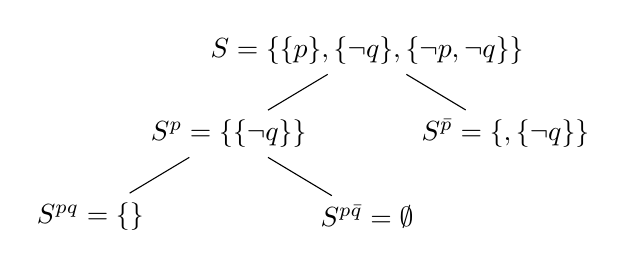
\begin{tikzpicture}[sibling distance=10em, level distance=3em]
  \node {$S = \{\{p\}, \{ \neg q\}, \{\neg p, \neg q\}\}$}
    child { node {$S^p = \{\{\neg q\}\}$} 
      child {node {$S^{pq} = \{\square\}$}}
      child {node {$S^{p\bar{q}} = \emptyset$}} 
    }
    child { node {$S^{\bar{p}} = \{\square, \{\neg q\}\}$}};
\end{tikzpicture}
\caption{An example of a reduction tree.}
\end{figure}

Interestingly, since $S$ can be infinite over a countable language, the tree can also be infinite. However, if $S$ is unsatisfiable, according to the compactness theorem, there is a finite $S' \subseteq S$ such that $S'$ is unsatisfiable. Therefore, after the reduction of all literals from $S'$, there will be $\square$ on every branch after finitely many steps.

Finally, we can prove the completeness of resolution. The theorem below shows completeness for finite formulas; the general version is obtained from that theorem by using compactness, similarly to the discussion of the reduction trees above.

\begin{theorem}[completeness of resolution]
If a finite $S$ is unsatisfiable, it is resolution refutable, i.e. $S \vdash_R \square$.
\end{theorem}
\begin{proof}
We will prove the theorem by induction on the number of variables in $S$. There is only one unsatisfiable $S$ without variables -- \{$\square$\} and therefore $S \vdash_R \square$ (the proof is the single step $\square$).

Let us now assume that $S$ is unsatisfiable and contains a literal $l$. Then by the previous lemma $S^l$ and $S^{\bar{l}}$ are unsatisfiable. These contain fewer literals than $S$ and therefore by induction there are resolution trees $T^l$ and $T^{\bar{l}}$ deriving $\square$ from $S^l$ and $S^{\bar{l}}$ respectively. Now, if every leaf of $T^l$ is in $S$, then $T^l$ is a resolution tree of $\square$ from $S$ and therefore $S \vdash_R \square$. Otherwise, we can append the literal $\bar{l}$ to each leaf of $T^l$ which is not in $S$ and to all of its predecessors, thus obtaining a resolution tree for $\{\bar{l}\}$ from $S$ (if the original leaf was not in $S$, the one with added $\bar{l}$ will be, as the only difference between $S^l$ and $S$ is the removal of $\bar{l}$). Similarly, by appending $\{l\}$ to leaves in $T^{\bar{l}}$ we obtain a resolution tree for $\{l\}$ from $S$. Resolving the roots of these trees yields a resolution tree of $\square$ from $S$.
\end{proof}

We have already mentioned that resolution is widely used in different automated systems -- SAT solvers, formal verification systems etc. One of the important examples is a Prolog interpreter. Prolog is a programming language where programs are sets of Horn clauses. The program can answer queries (goals). As Prolog programs are limited to Horn formulas, the resolution method can be improved. The Prolog interpreter uses so-called SLD-resolution which is based on LD-resolution and that is in turn based on LI-resolution, which is a special case of linear resolution. Therefore, we will now define linear resolution, show that LI-resolution is complete for Horn formulas and finally define LD- and SLD-resolution as simple improvements of LI-resolution.

\subsection{Linear resolution}

The general resolution procedure can be further simplified without losing the completeness. We define a linear proof of a clause $C$ from a formula $S$ as a finite sequence of pairs $(C_0, B_0), \dots, (C_n, B_n)$, such that $C_0 \in S$ and for every $i \leq n$, $B_i \in S$ or $B_i = C_j$ for some $j < i$, and $C_{i+1}$ is a resolvent of $C_i$ and $B_i$, where $C_{n+1} = C$. In the linear proof $C_0$ is called the \emph{starting clause}, $C_i$ a \emph{central clause}, and $B_i$ a \emph{side clause}. Again, we say that $C$ is \emph{linearly provable} from $S$ ($S \vdash_L C$), if it has a linear proof from $S$. A linear proof of $\square$ from $S$ is a \emph{linear refutation} of $S$ and $S$ is \emph{linearly refutable} if $S \vdash \square$.

Obviously, every linear proof can be transformed into a general resolution proof and therefore the linear resolution is also sound. Moreover, is is also complete (we omit the proof of completeness here).

%TODO: \add{Example of linear resolution}

\subsection{LI-resolution}

If we deal with Horn formulas, we can use an even more refined resolution procedure called linear input (LI) resolution. A LI-resolution from a formula $S$ is a linear resolution from $S$ where each side clause $B_i$ is from the input formula $S$ (i.e. $B_i$ cannot be a previously resolved central clause). We write $S \vdash_{LI} C$ to denote that $C$ is provable by LI-resolution from $S$.

We already defined Horn formulas while discussing the satisfiability problem. The definition from the resolution point of view is similar; the only difference is that we again use the set representation instead of the general one (and also formulas in this case can be infinite, as there is no distinction between theories and formulas in resolution). So a \emph{Horn clause} is a finite set of literals containing at most one positive literal. A Horn formula is then a (potentially infinite) set of Horn clauses. A clause \{p\}, where $p$ is a positive literal is called a \emph{fact}, and a clause with exactly one positive literal is called a \emph{rule}. Rules and facts are also called \emph{program clauses}. A non-empty Horn clause without any positive literal is called a \emph{goal}.

We can easily see that if a Horn formula $S$ is unsatisfiable and it does not contain $\square$, it must contain some fact and some goal. Why? If $S$ does not contain any fact, it is satisfied by setting all the propositional variables to 0. if it does not contain any goal, it is satisfied by setting all variables to 1.

LI-resolution is complete for Horn formulas, as the following theorem says. The proof of the theorem is similar to the proof of completeness of general resolution.

\begin{theorem}[completeness of LI-resolution]
If $T$ is a satisfiable Horn formula but $T \cup \{G\}$ is unsatisfiable for some goal $G$, then $\square$ has an LI-resolution from $T \cup \{G\}$ with starting clause $G$.
\end{theorem}
\begin{proof}
As in the proof of completeness of general resolution, we use induction on the number of variables, this time in $T$. By the observation above, $T$ must contain a fact $\{p\}$ for some variable $p$ ($T \cup \{G\}$ is unsatisfiable, therefore it must contain a goal and a fact; $G$ is a goal, so the fact must be in $T$). By the lemma we used in the proof of completeness of general resolution, $T' = (T \cup \{G\})^p = T^p \cup \{G^p\}$ is unsatisfiable and $G^p = G \setminus \{\neg p\}$. Now, if $G^p = \square$, we have $G = \{\neg p\}$ and thus $\square$ is a resolvent of $G$ and $\{p\}\in T$. Otherwise, since $T^p$ is satisfiable (by the satisfying assignment for $T$) and has fewer variables, by the induction assumption, there is an LI-resolution of $\square$ from $T'$ starting with $G^p$. If we now append the literal $\neg p$ to all leaves that are not in $T \cup \{G\}$ (and their predecessors), we have an LI-resolution proof of $\{\neg p\}$ from $T$; we can resolve it with $\{p\}$ from $T$ to obtain the LI-resolution proof of $\square$ from $T$.
\end{proof}

\subsection{Resolution in Prolog}

A program in Prolog is a set of program clauses (i.e. rules or facts). An example program is shown below (the program contains seven clauses; the numbers indicate line numbers and are not part of the program):

\begin{verbatim}
1: p:-q,r.                    5: r.
2: p:-s.                      6: s:-t.
3: q.                         7: s.
4: q:-s.
\end{verbatim}

The formulas on lines 3, 5, and 7 are facts, the rest are rules. The symbol \texttt{:-} can be interpreted as an implication from right to left ($\leftarrow$). So the meaning of the clauses is as given below:

\begin{multicols}{2}
\begin{enumerate}
  \item $q \land r \to p$
  \item $s \to p$
  \item $q$
  \item $s \to q$
  \columnbreak
  \item $r$
  \item $t \to s$
  \item $s$
\end{enumerate}
\end{multicols}

In Prolog, we want to know whether a query is a consequence of a given program. A query is a conjuction of goals (positive literals), e.g. $p \land q$. That means that the question is whether for a program $P$ and query ($q_1 \land \dots \land q_n$) it holds that $P \vDash (q_1 \land \dots \land q_n)$. However, such a question is equivalent to the fact that $P \cup \{\neg q_1, \dots, \neg q_n\}$ is unsatisfiable, which is equivalent to $\square$ having an LI-resolution from $P \cup \{G\}$ starting with the goal $G = \{\neg q_1, \dots, \neg q_n\}$.

In the Prolog interpreter, the clauses are represented as sequences of literals (as opposed to sets of literals as in LI-resolution). Therefore, Prolog uses a slightly different version of LI-resolution called LD-resolution (linear definite). In LD-resolution, the resolvent of a goal $(\neg p_1, \dots, \neg p_{i-1}, \neg p_i, \neg p_{i+1}, \dots, \neg p_n)$ and a rule $(p_i, \neg q_1, \dots, \neg q_m)$ is a new goal $(\neg p_1, \dots, \neg p_{i-1}, \neg q_1, \dots, \neg q_m, \neg p_{i+1}, \dots, \neg p_n)$, i.e. one of the negative literals in the current goal is replaced by the negative literals from the rule. 

LD-resolution does not specify which of the negative literals in the goal should be resolved next. This would make programming in Prolog hard, therefore it extends the LD resolution with a selection rule $\mathcal{R}$. Typically, the rule is ``select the first literal''. More formally, an SLD-resolution via $\mathcal{R}$ is an LD-resolution in which we resolve each step $(C_i, B_i)$ through $\mathcal{R}(C_i)$.

Obviously, any LI-resolution can be expressed as an LD-resolution (just use the sequences of literals instead of the sets of literals), and any LD-resolution can be expressed as an SLD-resolution with the correct selection rule
 (select the literal that was selected in the LD resolution). Therefore, we can see that SLD resolution is complete for Prolog programs.

Further discussion of Prolog is out of the scope of this lecture, so we will omit it here. The important message was to show an application of logic in computer science. Prolog is quite often used in certain areas of artificial intelligence.

\bigskip

This concludes the part of the lecture dedicated to propositional logic. We started with a discussion about the syntax of propositions, explained their semantics and showed some formal proof systems. In the next part of the lecture, we will build on our understanding of concepts from  propositional logic and extend them to predicate logic (more precisely to first-order logic).
